\chapter{The \nova~Experiment}
\label{ch:nova}

The \nova~experiment, or the NuMI Off-Axis $\nue$ Appearance experiment, is a long baseline, two detector, neutrino oscillation experiment designed to measure $\numu$ to $\nue$ appearance from the Fermilab NuMI beam. The two functionally identical \nova~detectors are situated $14.6\unit{mrad}$ off-axis of the beam center, with its Near Detector (ND) located approximately $1\unit{km}$ downstream of the beam target source and its Far Detector (FD) located $810\unit{km}$ from the source in Ash River, MN. The main purpose of the ND is to constrain the neutrino beam energy and composition by measuring the beam very close to its source, i.e., before the neutrinos have had a chance to oscillate. The FD then measures the oscillated neutrinos. This chapter describes the NuMI beam and \nova~detectors in more detail.

\section{The NuMI Beam}

The NuMI beam is a $\numu$ beam generated at Fermi National Accelerator Laboratory, or Fermilab, in Batavia, IL, and the source of neutrinos for the \nova~experiment. The neutrino beam is created by accelerating protons to $120\unit{GeV}$, colliding them with a fixed target, and allowing the products to decay to neutrinos.

The NuMI beam originates with the $120\unit{GeV}$ protons, and these are accelerated in the complex shown in figure \ref{fig:FNAL_AC}. First, negatively charged hydrogen atoms are accelerated to $400\unit{MeV}$ in the Linac. These atoms next enter the Booster synchrotron where the electrons are removed and the protons are accelerated to $8\unit{GeV}$. The output of from the booster is $13$ bunches, $12$ which are extracted into the Recycler Ring, each with approximately $4\times10^{12}$ protons. In a procedure called slip stacking, additional bunches are used to double the intensity of each bunch. The first bunches in the Recycler are decelerated slightly while $6$ new bunches enter the ring. As the two sets of bunches have slightly different energies, they slip relative to each other. When two bunches overlap they are captured with a special RF pulse, creating $6$ larger bunches that are extracted into the Main Injector (MI) and accelerated to $120\unit{GeV}$. Finally, these protons are directed to the fixed target for neutrino production. At this point, the 6 bunches, or the spill, total about $5\times10^{13}$ protons. With a cycle time of $1.333\unit{s}$, the NuMI beam reaches $700\unit{kW}$, which is the most powerful beam in the world \cite{ref:TDRNOvA}.
\begin{figure}[htb]
  \centering
  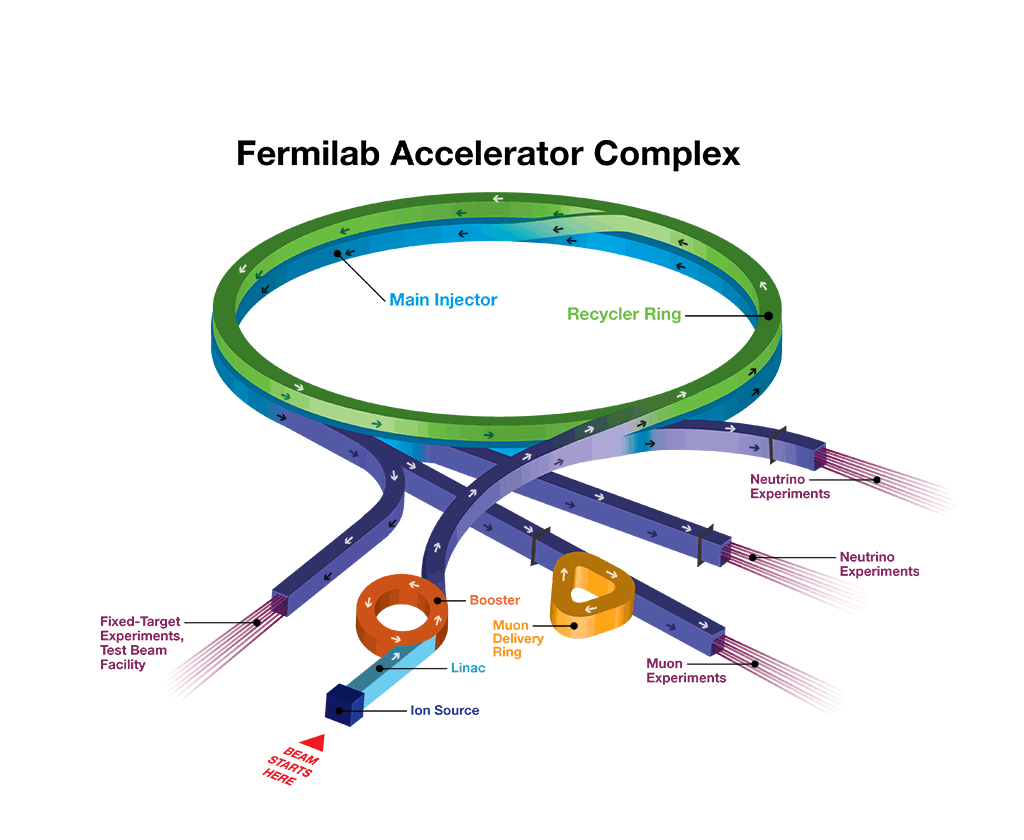
\includegraphics[width=0.75\textwidth]{figures/FNAL_AC.png}
  \caption[Fermilab Accelerator Complex]{Schematic of the Fermilab accelerator complex.}
  \label{fig:FNAL_AC}
\end{figure}

In truth, the above is the design goal of the NuMI beam upgrades. The NuMI beam was originally designed for the MINOS experiment \cite{ref:TDRNuMI}, and it was operating at ${\sim}200\unit{kW}$ with no slip stacking at the time of writing the \nova~Technical Design Report (TDR) in 2007 \cite{ref:TDRNOvA}. Since then, the Fermilab Accelerator Division has been steadily ramping up the beam power, as shown in figure \ref{fig:BeamPower}. At the time of writing of this dissertation, the NuMI beam was in the midst of its 2016 summer shutdown. Before the beam was powered down, it most recently was running stably at about $560\unit{kW}$ with $6{+}4$ slip stacking, or doubling the proton intensity in just $4$ of $6$ bunches \cite{ref:IntensitykW, ref:IntensitySlip}. However, the NuMI beam briefly reached its design goal of $700\unit{kW}$ with full $6{+}6$ slip stacking during a test on June 13, 2016 \cite{ref:Intensity700}.
\begin{figure}[htb]
  \centering
  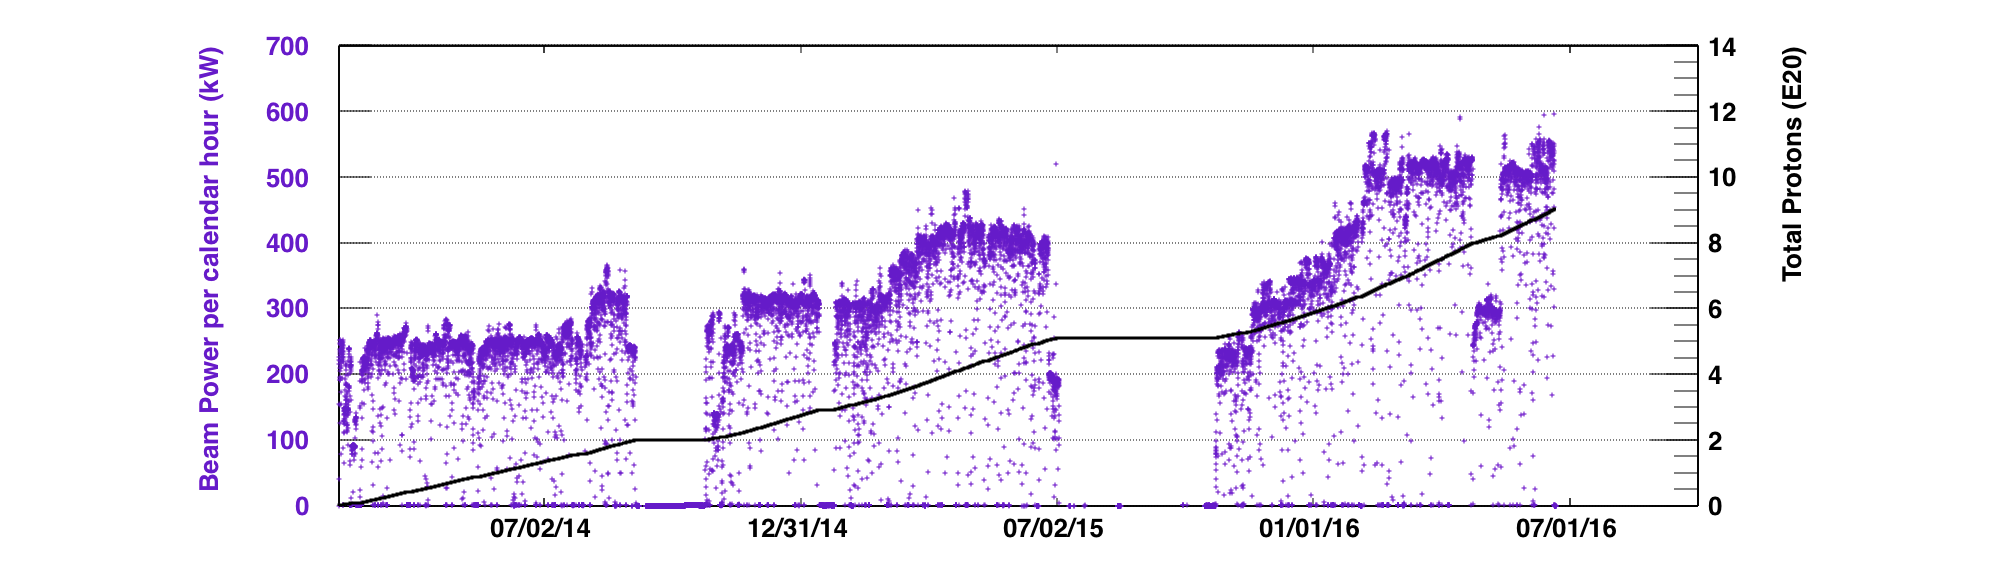
\includegraphics[width=1\textwidth]{figures/BeamPower.png}
  \caption[Beam Power vs Time]{Beam power vs time since \nova~began collecting data. The average beam power is shown as purple points, and the integrated POT is shown in the black curve.}
  \label{fig:BeamPower}
\end{figure}

\section{The \nova~Detectors}

\subsection{Near Detector}

\subsection{Far Detector}